\section{Challenge I: Establishing Body Movement Patterns as Reliable Features for Authentication}\label{sec:learning}

Even though body movements have been deemed unique by human brains for a long time, the need to capture the signal and quantify its uniqueness using wearable device is highly challenging. In this section, we present our proposed techniques to address this challenge.

\subsection{Preliminary Results}
We have conducted a preliminary study to find out whether body movements measured by wearable devices can potentially be used for robust authentication.
In our preliminary study, we used Google glass to collect accelerometer data ($ACC$ in short) when a user moves her head following music beats, and studied whether the measured head movement patterns are distinctive and repeatable. Our preliminary study involves the following data processing aspects:

\begin{enumerate}
\vspace{-2pt}\item \emph{Filtering}: Since the frequency spectrum of the $ACC$ samples is significantly concentrated within 5Hz, we filtered the raw samples using a low-pass digital Butterworth filter~\cite{challis1983design} by adopting a relaxed cut-off frequency of 10Hz. In this way, we removed spurious head movements and obtained smooth $ACC$ data.

\vspace{-2pt}\item \emph{Reference Data Construction:} We constructed the reference data set to include $m$ $ACC$ samples from the legitimate user (which we refer to as \emph{true} $ACC$ samples), as well as $m$ $ACC$ samples each from $N$ random users (referred to as \emph{false} samples). Then we calculated the distances between these samples using the dynamic-time warping (DTW) tool~\cite{dtw}\footnote{DTW is generally used to measure similarity between temporally varying signals. DTW compares a temporal signal with a reference signal over a certain time-window and calculates the distance between these two signals.}. Using DTW, we calculated the distances between true $ACC$ samples and the distances between true samples and false samples, and refer to these two types of signatures as same-user distance signatures as well as across-user distance signatures. In general, we find that same-user distances are much smaller than cross-user distances. 

\vspace{-2pt}\item \emph{SVM Classification:} In the online authentication phase, after filtering the raw $ACC$ signal, we calculated the DTW distances between the test sample and the true samples, and then feed these distance values and the reference data to the Support Vector Machine (SVM) to obtain classification results. %SVM returns '1' to denote that the test user is accepted and '0' to denote the user is rejected.

\end{enumerate}


\begin{table}[b]
\centering\small
\begin{tabular}{|l||l|l|l||l|l|l||l|l|l||l|l|l|}\hline
& \multicolumn{3}{|c||}{2}& \multicolumn{3}{|c||}{3}& \multicolumn{3}{|c||}{6}& \multicolumn{3}{|c|}{10}\\\cline{2-13}
Sample duration (s)& FRR & FAR & BAC & FRR & FAR & BAC & FRR & FAR & BAC & FRR & FAR & BAC\\
&(\%) &(\%) &(\%) &(\%) &(\%) &(\%) &(\%) &(\%) &(\%) &(\%) &(\%) &(\%)\\\hline

SVM          & 25.0 & 16.74 &79.12 & 15.0 & 14.05 & 85.47 & 3.33& 6.66& 95.0  & 0.0& 9.62& 95.18\\\hline

\end{tabular}
\caption{Average FAR, FRR, and BAC for SVM-based classification in our preliminary study. The results show that even for the simplest nodding, we can correctly authenticate 95\% of the users when the samples are longer than 6 seconds. \label{tab:kfoldfalse-svm}}
\end{table}


\vspace{4pt}\textbf{Distinctiveness:} We designed the first set of experiments to show that even the simplest head movements are distinctive -- i.e., it is hard to imitate other's movement patterns. In this set of experiments, we employed the simplest head movement pattern: nodding. In total, we had one glass owner, who designed the nodding pattern, and 15 imitators who imitated the pattern. We collected 100 10-second $ACC$ samples from the owner, during the course of 60 days (from 10/1/2014 to 11/30/2014), ensuring the owner's sensor data includes sufficient variation that naturally arises with time. We also made a great deal of effort to make sure the imitators accurately copy the owner's movement -- the owner carefully explained how he nodded his head to each imitator, and sat through each data collection session for all the 15 imitators to make sure their nodding patterns look the same to the owner's eye. For each imitator, we collected 40 10-second $ACC$ samples. By averaging over many different combinations of reference data and test data, we generated the average classification results and summarized the mean FAR (false acceptance rate), FRR (false rejection rate), and BAC (balanced accuracy) in Table~\ref{tab:kfoldfalse-svm}. The results show that \emph{even simple nodding is not easy to imitate: nodding for 6 seconds can help classify 95\% of the users.} %As the sample duration increases from 2 seconds to 6 seconds, the classification accuracy improves significantly -- the BAC value changes from 79.12\% to 95\% for top 1 testing, and from 87.95\% to 93.27\% for top 3 voting. After the sample duration reaches 6 seconds, the improvement becomes less pronounced. This suggests that a sample duration of 6 seconds is sufficient to successfully classify 95\% of the users. We feel that moving our head gently along with music for 6 seconds is in general not a cumbersome process for most users. It further suggests that even simple nodding is hard to imitate by others, and thus head-movement has the potential to %serve as a reliable biometric characteristic for smart wearable authentication.

\begin{figure*}[t]
\centering
\includegraphics [width=.75\linewidth]{../mobisys_paper/fig/exp2_frr_far_bac.pdf}
\caption{In this set of experiments, we studied whether a user can successfully repeat her own head-movement pattern. We had 8 subjects, each performing her own choice of head-movement patterns. We collected 38 samples for each subject. (a) shows the FRR and FAR results for each subject, and (b) shows the BAC results.\label{fig:exp2_frr_far_bac}}
\end{figure*}

\vspace{4pt}\textbf{Repeatability:} We designed the second set of experiments to show that a user can successfully repeat her own head movement pattern if each user is asked to come up with their own movement pattern. In this set of experiments, we had 8 subjects, and for each subject, we collected 38 $ACC$ samples with sample duration of 10 seconds. Each subject performed different head-movement patterns of their choice. We report the average FAR, FRR, and BAC values in Figure~\ref{fig:exp2_frr_far_bac}, where Figure~\ref{fig:exp2_frr_far_bac}(a) shows the FRR and FAR values, while Figure~\ref{fig:exp2_frr_far_bac}(b) shows the BAC values. The results show that \emph{head-movements are highly repeatable.} Among the 8 subjects that we studied, the highest BAC value is 100\%, and the lowest is 91.81\%, with the average BAC value of 95.57\%.

%Overall, our preliminary results suggest that the head movement pattern is a very promising biometric candidate for wearable user authentication.

\subsection{Proposed Research}
Our preliminary results show that simple movement patterns have the potential to be used as a reliable biometric characteristic for wearable user authentication. However, in order to develop a full-fledged authentication system using free-style body movements, we need to eliminate several important roadblocks.

\subsubsection{Feature Selection and Information Entropy}\label{sec:feature}
Feature selection plays the most important role in determining the accuracy of an authentication system, and we will thus start our discussion from this topic.  Most wearable devices have accelerometer ($ACC$) and gyroscope ($GYRO$) sensors, whose readings can be used to characterize a person's body movements. There has been a long history of studying these two types of sensor data to detect/analyze motion, and a large number of features have been discussed~\cite{palmerini2011feature,Pirttikangas2006feature,preece2009comparison,bao2004activity,zhang2011feature}. In this project, we will start our investigation by evaluating these features, and propose to look at the following features in depth: (1) mean, standard deviation, median, 25\%, and 75\% of frequency (in the frequency domain), (2) mean low and mean rectified high pass filtered signals (in the frequency space), (3) centroid frequency (in the frequency domain), (4) frequency dispersion (in the frequency domain), (5) power spectrum of entropy in acceleration/rotation and average energy in acceleration/rotation (in the frequency domain), (6) magnitude of first five components of FFT analysis (in the frequency domain), (6) jerk index that indicates the smoothness of the signal (in the time domain), (7) mean crossing (in the time domain), (8) maximum difference acceleration (in the time domain), (9) correlations between axes (in the time domain). We will conduct an in-depth comparison of these features, and select those that deliver the best performance; meanwhile, we will also design new features that are suitable for our study.

\vspace{4pt}\textbf{Boosting Information Entropy:} It is important to encode as much information as possible into the observed sensor signals to achieve higher information entropy. One way of achieving this goal is to have the user move her body naturally following an external music stimulus -- we hypothesize that different people translate music stimuli to motor movements in different ways~\cite{bartenieff1980body,brass2001movement,dassonville2001effect}. For example, some people are able to follow beats much closer than others, some can follow beats more regularly than others, etc. By using the music stimuli, in addition to the afore-mentioned baseline $ACC$/$GYRO$ features, we can also consider a group of new features concerned with the temporal relationship between music beats and subsequent body movements --  such as mean and standard deviation of the intervals between a music beat and the subsequent body movement, the top interval values, etc. In this way, the sensor data contains more information than just the movement pattern.

In order to further boost the information entropy, we can also switch the music track during a data collection session. In this way, the sensor data does not only contain the user's motor response to the music beats in a steady state, but it also encodes information about how fast the user adapts to the change of music rhythm, which provides more discrimination power.

\subsubsection{User Authentication Through Combined Movements and Sensors}

Smart wearable devices typically contain an array of motion sensors such as accelerometer, gyroscope, and inertial measurement unit (IMU). It is only a matter of time that motion sensor chips will be integrated into wearable devices.
This opens up opportunities for multi-modal motion sensing. For example,
accelerometer data can be combined with gyroscope measurements to provide
multi-dimensional movement features that can improve the quality of the
inferred signatures. Head movements can also be combined with other body movements to generate
valuable, reliable signatures for authentication. In this project, we plan to explore these opportunities.
%Additionally, head-movement is just one type of body movements, and we can
%investigate other types of body movements as well.


\begin{wrapfigure}{r}{3.0in}\centering
\vspace{-12pt}
\begin{tabular}{cc}
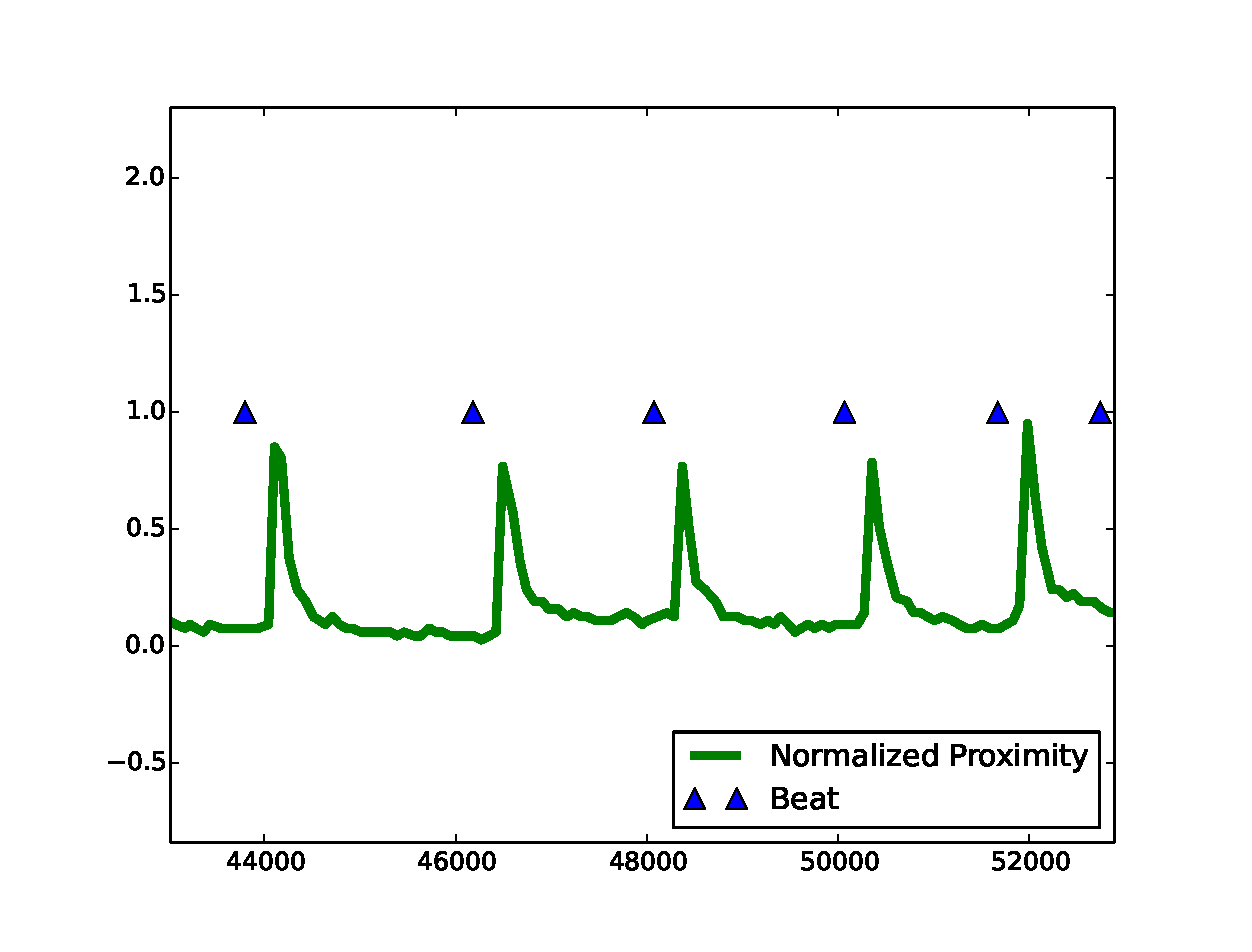
\includegraphics[width=0.50\linewidth]{../figure/sub1_blink_beat} &
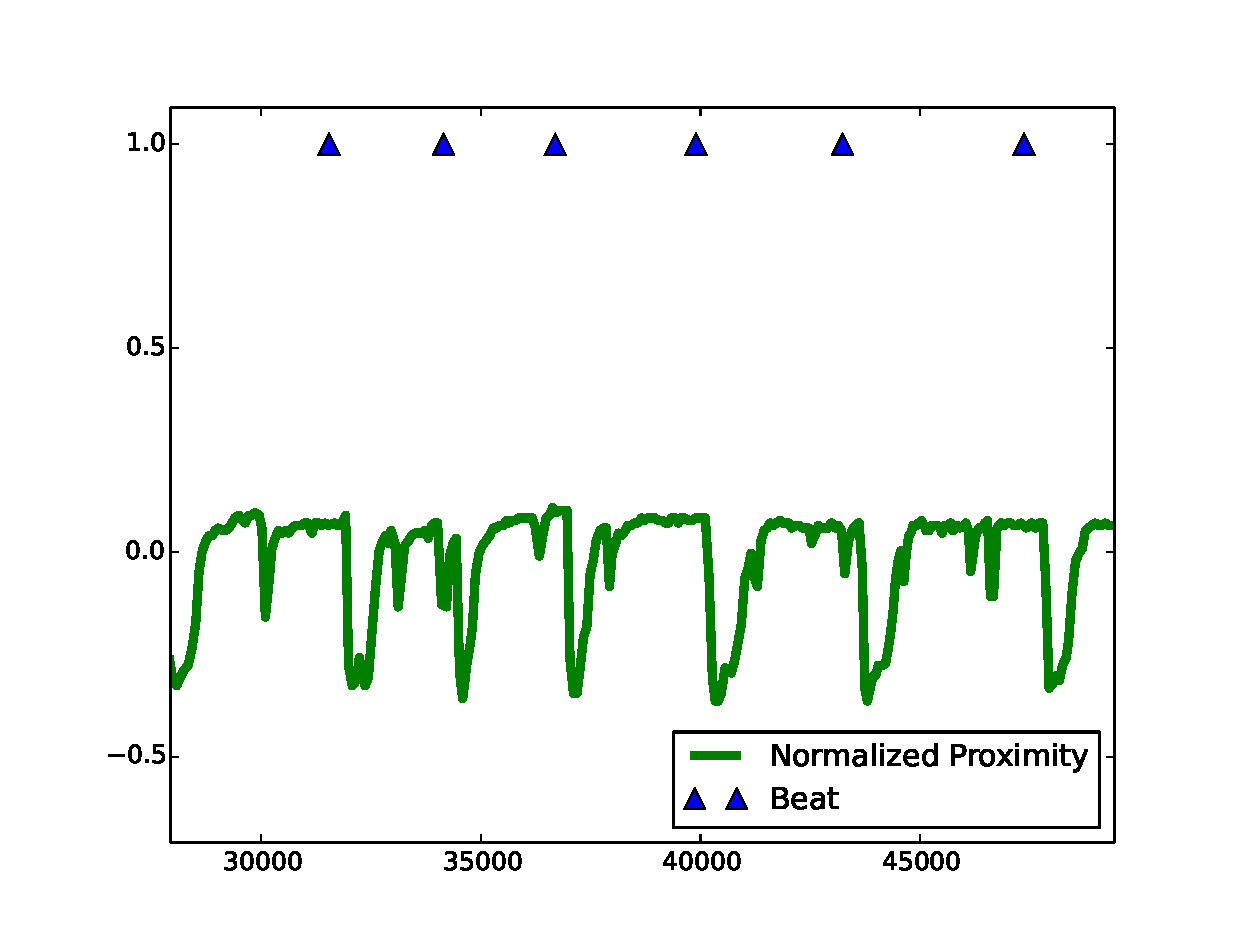
\includegraphics[width=0.50\linewidth]{../figure/sub2_blink_beat} \\
(a) & (b)\\
\end{tabular}
    \caption{\label{fig:blink} A person's blinking patterns (measured by the infrared proximity sensor on the Google Glass) with respect to music beats are also differentiable.}
\vspace{-12pt}
\end{wrapfigure}
\vspace{4pt}\textbf{Combining Multiple Movement Signatures:} In our preliminary study, we only looked at monitoring head movements for authenticating Google Glass. In reality, there are other types of movements that can be captured by Google Glass for authentication purposes. For example, through a simple test experiment using the Google Glass
infra-red light sensor we observed that the blinking and winking patterns of users in
response to the music can be combined with head-movements for better results. For example, Figure~\ref{fig:blink} shows two users' blinking pattern (captured by the infra-red light sensor, or the proximity sensor) with respect the music tones are vastly different. Recent studies have also shown that heart beat or pulse can be read by Google Glass~\cite{hernandezbioglass}. In this project, we will look at whether these signals can be combined to obtain better classification results.

The main challenge in combining multiple movements stems from the fact that it is hard to separate their impacts on motion sensor readings (e.g, the fact that a user winks may change the way she moves her head). As a result, if not properly handled, combining movements may actually worsen the authentication results. In this project, we will carefully investigate what new features we will exploit if multiple movement patterns are combined.

\vspace{4pt}\textbf{Combining Accelerometer and Gyroscope:} Quite a few previous studies have looked at combining accelerometer and gyroscope readings to detect motion contexts such as walking, standing or fall~\cite{mayagoitia2002accelerometer,jovanov2005wireless,li2009accurate,zhu2004real,williamson2001detecting,sabatini2005assessment}. In our preliminary study, however, we find that gyroscope data from Goolge Glass fared very poorly in discriminating users' head movements. The reason is that gyroscope often drifts over time. Low pass filtering can help cancel such drifts, but it also erases much useful information in the low frequency range, thus rendering it less useful. On the other hand,  complimentary filters (discuss in~\cite{euston2008complementary}) that combine accelerometer and gyroscope readings could provide attitude estimation. It performs low-pass filtering on a low-frequency attitude estimation that is obtained from accelerometer, and high-pass filtering on a high-frequency attitude estimation that is obtained by the integration of  gyroscope data. Though better than low-pass filtering alone, this may also lead to information loss in the low frequency range, hence poorer classification results. In this project, we will try to develop a signal processing method that can better preserve information in the low-frequency range.

\vspace{4pt}\textbf{Authenticating Multiple Devices:} When a person has multiple wearable devices, we don't need to authenticate the same user to different devices one by one (assuming these devices are not put on at the exactly the same time). Instead, after the user is authenticated on the first device, the first can help the user authenticate on the second device by having the user make simple and short body movements that can be measured by both devices (e.g., shaking two devices using one hand each)~\cite{mayrhofer2007shake,patel2004gesture}.


\subsubsection{Robust Authentication in Mobile Settings}
Our preliminary results show that head movements are rather distinctive and repeatable in very controlled settings -- all the data were collected when the participant was in a stationary setting, i.e., sitting on a chair. However, in reality, the behavior of body movement signatures over chaotic settings will be a key factor to decide on the effectiveness of this approach. In this project, we strive to solve the challenge for the most common mobile setting: when the user is walking.
%Our work only evaluates the case when a
%user is in a stationary setting when attempting to login, such as when sitting
%on the chair or standing still. The performance of this approach in realistic


\begin{wrapfigure}{r}{4.0in}\centering
\begin{tabular}{cc}
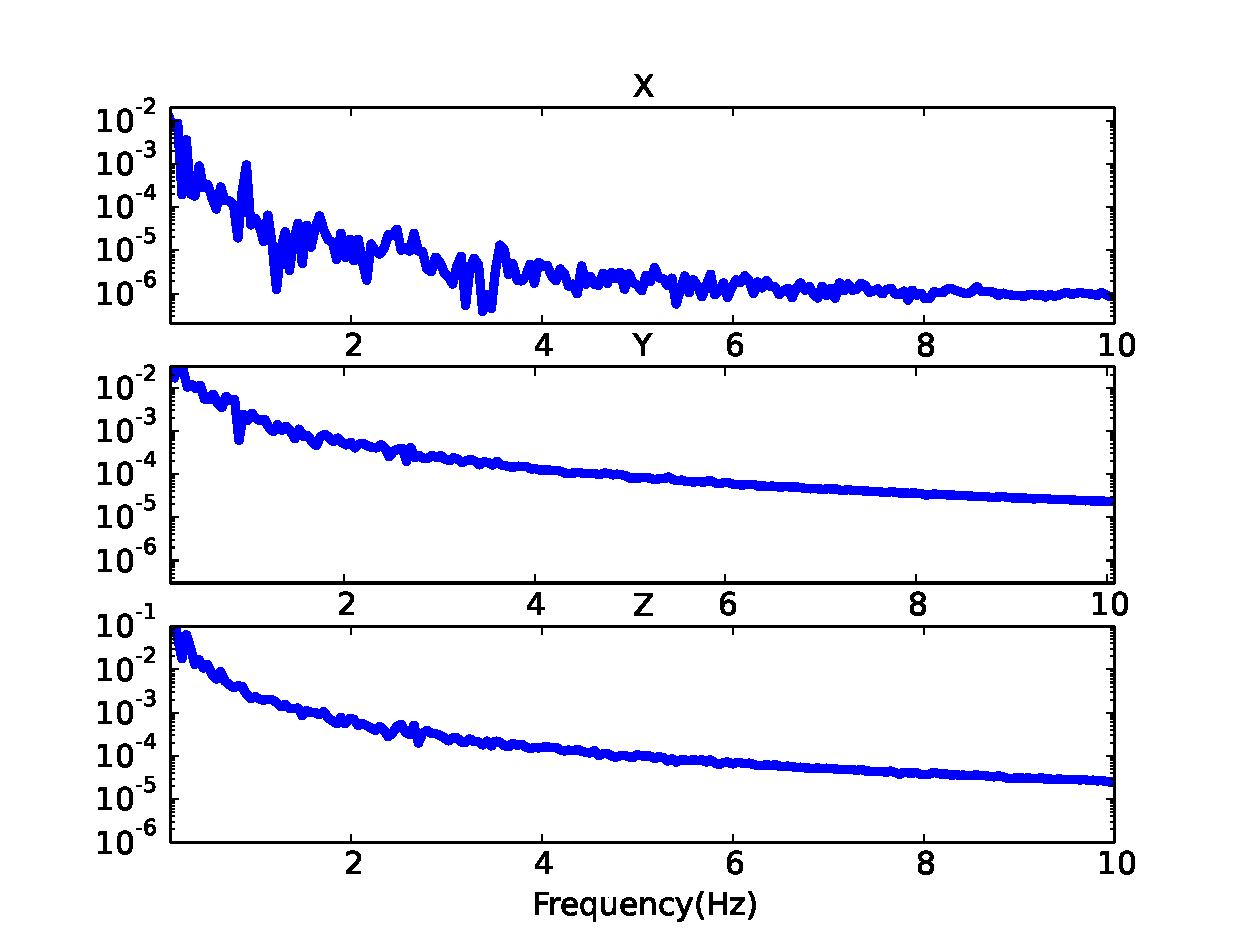
\includegraphics[width=0.50\linewidth]{../figure/sub1_walking_freq} &
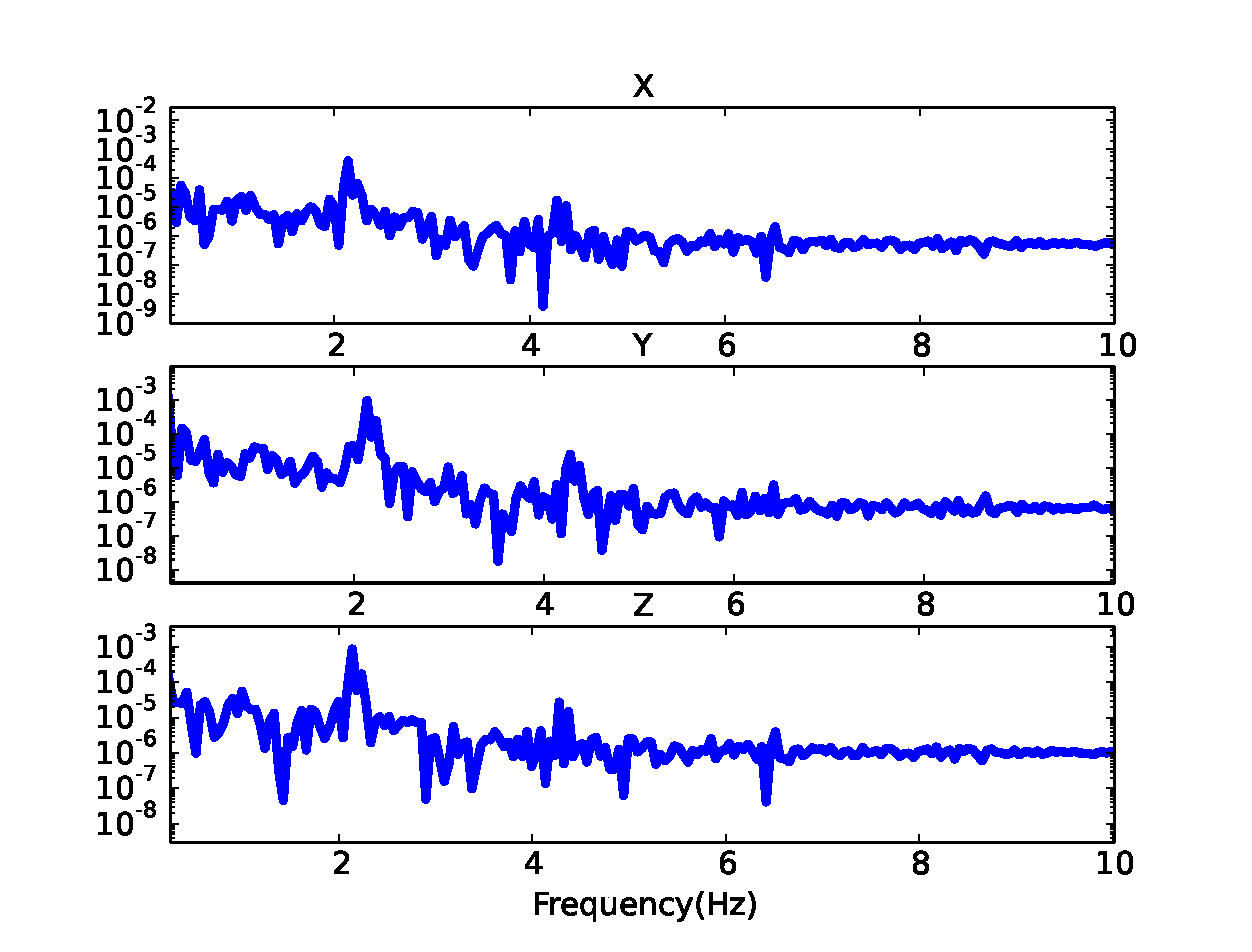
\includegraphics[width=0.50\linewidth]{../figure/sub1_nodding_freq} \\
(a) & (b) \\
\vspace{-4pt}
\end{tabular}
    \caption{\label{fig:walk} Walking (a) usually has more energy than music-stimulated partial body movement such as nodding (b).}
\vspace{-6pt}
\end{wrapfigure}
\vspace{4pt}\textbf{Authenticating Walking Users:}  For a walking user, we can't rely on the original training data that is collected when the user was sitting or standing still any more; performing body movements while walking will definitely lead to different movement signatures.

When considering walking, we can collect sensor readings in three different scenarios (we only focus on $ACC$ data in this part for the sake of simplicity): ${ACC_{M+W}}$, denoting the sensor readings when the user is performing body movements while walking; ${ACC_{M}}$, denoting the sensor readings when the user is performing body movements while sitting or standing still; and ${ACC_{W}}$, denoting the sensor readings when the user is walking, without any special body movements. To address the challenge of authenticating walking users (whose test data is $ACC_{M+W}^{tst}$), a naive
method is to use an external accelerometer (such as the one on the smartphone) to record the motion caused by walking ($ACC_{W}^{tst}$). We can then extract the motion caused by special music-stimulated body movements as $$ ACC_{M}^{tst} = ACC_{M+W}^{tst} - ACC_{W}^{tst}.$$ Finally we can compare $ACC_{W}^{tst}$ with the reference data $ACC_{W}^{ref}$ to classify the user. Though simple and effective, this method does require another device, which is less convenient, as we have argued before. As a result, we will \emph{not} adopt this method in the project.


If we only use the accelerometer on the device, authenticating a walking user becomes much harder, mainly because a person's walking pattern is much less repeatable -- factors such as trajectory, speed, terrain will have a bearing on the walking pattern -- and the interaction between walking and music-stimulated body movements are very complex and hard to predict. Due to the complexity of this problem, we will explore a learning-based authentication approach. In the learning phase, the system will ask the user to perform the designed body movements while she is in different walking contexts (walking in office, walking at home, walking on the parking lot, etc.). The system will then run clustering algorithms on the collected accelerometer data, and cluster them into a small number of groups, representing the data within her typical walking contexts. For each such group, we maintain a certain number of reference data.

In the classification phase, we adopt a two-level classifier. At the top level, we determine whether the user is stationary or mobile. This is rather straightforward because walking in general has much more energy than music-stimulated body movements as shown in Figure~\ref{fig:walk}. At the bottom level, if the user is walking, we classify the test data against the user's walking reference data group by group. If none of the groups return TRUE, we reject the user.


\subsubsection{Stronger Authentication Through Body Movement Based Passwords}\label{subsec:password}
Like any behavioral biometric characteristic, the body movement pattern may fail to differentiate users in some cases. For those users who desire a more secure authentication method, we propose to use movement-based passwords, which offers more security, reduces the processing demands on the device, but requires the user to remember their passwords.

Like traditional text passwords, body movement passwords also contain a list of elements -- how many elements are in the password and what they are determine the password. However, unlike tradition passwords in which each element is a character, each element of the body movement passwords is a type of body movement. For example, a password for a smart glass user can have the following four movements: a head nod, an eye blink, a head nod, and a head shake; a password for a smart watch user can have the following four movements: upward movement, right-award movement, left-award movement, and downward movement. For each element, the system also designs a unique prompt tone that the user needs to remember. 

The proposed password-based authentication system works as follows. First, we ask the users how many elements are contained in her password. Then for each element, the system will play a tone to mark the beginning of the element. We make sure two consecutive tones will be reasonably apart so that the user has sufficient time to finish each movement. In this case, the system doesn't need to differentiate users solely based upon their movement signatures, but the system only needs to recognize the movement. We will also provide a list of supported movements such as a head nod, a head shake, or an eye blink. Finally, for each authentication session, the system plays the prompt tones in a \emph{random} order to avoid shoulder surfing. Compared to using body movements as biometrics, this method is simpler, more secure, and easier to reconfigure than purely movement pattern based authentication. 


